\documentclass[12pt,oneside,listof=totoc,paper=a4,headings=small]{scrbook}
% Nützliche Packages für die Gestaltung und allgemeine Konfiguration des Dokuments
% -----------------------------------

% Allgemeine Formatierungen
\usepackage[ngerman]{babel}			% neue deutsche Rechtschreibung
\usepackage[utf8]{inputenc} 		% Umlaute im Text
\usepackage[T1]{fontenc}
\usepackage{xspace}                 % Vermeidung von "ineinanderfallenden f's", wie z.B. bei Schifffahrt
\usepackage{url}		            % korrekte Anzeige/Umbruch von URLs
\usepackage{listings}               % z.B. nützlich zum Einbinden von Quellcode
\usepackage{hyperref} 				% für Hyperlinks in PDF-Dokumenten 
\usepackage{lmodern}
\usepackage{enumitem}
\usepackage{csquotes}
\usepackage{tabularray}
\usepackage{xcolor}
\usepackage{caption}
\captionsetup[wrapfigure]{format=plain, justification=justified, singlelinecheck=false}
\setlist{noitemsep}

\usepackage{wrapfig}

\usepackage{tocbibind}

\usepackage{subcaption}

\definecolor{bg}{rgb}{0.95,0.95,0.95}

\usepackage{minted}
\setminted{
	fontsize=\footnotesize,
	linenos,
	bgcolor=bg,
}
\usepackage{tcolorbox}

% Kopfzeile
\usepackage[headsepline,manualmark]{scrlayer-scrpage}
\clearpairofpagestyles
\ohead{\pagemark}
\ihead{\headmark}
\automark{chapter}
\pagestyle{scrheadings}

% Seitenspiegel
\usepackage[left=25mm,right=20mm,top=25mm,bottom=25mm]{geometry}

% Literatur
\usepackage[backend=biber, %% Hilfsprogramm "biber" (statt "biblatex" oder "bibtex")
            style=numeric, %% Zitierstil (siehe Dokumentation, bitte mit Betreuer absprechen)
            natbib=true, %% Bereitstellen von natbib-kompatiblen Zitierkommandos
            hyperref=true, %% hyperref-Paket verwenden, um Links zu erstellen
]{biblatex}

% Einbindung der Literatur-Datenbank
\addbibresource{./Literatur/quellen.bib}

% Grafiken
\usepackage{graphicx} 				% Grafiken einfügen (pdf,png - aber jpg vermeiden)
\graphicspath{{./Bilder/}}          % Pfad zu den Bildern
\usepackage{lipsum}                 % For placeholder text, you can remove this and add your text

% Tabellen
\usepackage{booktabs} 				% bessere Gestaltung von Tabellen
\usepackage{longtable} 				% für bessere Tabellen über mehrere Seiten

% Koma-Script Kompatibilität
\usepackage{scrhack}

% 1.5 Zeilenabstand
\usepackage{setspace}
\onehalfspacing

% Das Dokument selbst mit seinen Bestandteilen
% --------------------------------------------
\begin{document}
\frontmatter 
    % Titelseite soll keine Kopf oder Fußzeile haben
\thispagestyle{empty}



\vspace*{-20mm}
\begin{flushright}

\includegraphics[width=0.5\textwidth]{Bilder/LogoHS.png}
\end{flushright}


\vspace*{2cm}

% Alle Elemente sollen zentriert sein
\begin{center}
% Art der Arbeit => (Bachelorarbeit , Masterarbeit, Studienarbeit)
{\Large \textbf{Seminar}}\\ 



\vspace{1cm}

% Titel der Arbeit 
{\Large \bfseries Refactoring in der Softwareentwicklung\\ 
	Sommersemester 2024\\
	bei Prof. Dr. Georg Hagel\\}

\vspace*{1cm}

{\large five lines of code (Christian Clausen)\\[1mm]}

\vspace{1.5cm}

% Name des/der Autors/Autoren
{\large Thema: Fogle der Struktur im Code}\\[40mm]

\end{center}

\vfill

% Aufgabensteller, Kontaktdaten und Abgabetermin
\parbox{120mm}{
\begin{tabbing}
Name, Vorname \hspace{2cm} \= Heiserer Valentin\\
Matrikelnummer             \> 453990\\[4mm]
Studiengang                  \> Bachelor Informatik\\
Semester                  \> Sommersemester 2024\\
\end{tabbing}
}

 				    % Titelblatt
%    \newpage
\thispagestyle{empty}

% Bitte hier keine Änderungen vornehmen, sondern vollständig handschriftlich ausfüllen

\noindent  {\Large \textbf{Sperrvermerk}}\\ 

\vspace*{2cm}
\bfseries
\noindent Die nachfolgende Arbeit enthält vertrauliche Informationen und Daten der Firma
VeryBest GmbH. 

\medskip
\noindent Veröffentlichungen oder Vervielfältigungen - auch nur auszugsweise oder in
elektronischer Form - sind ohne ausdrückliche schriftliche Genehmigung der
Firma VeryBest GmbH nicht gestattet.
\medskip

\noindent Die Sperrfrist gilt bis zum 31. Dezember 20XY.

\medskip
\noindent Die Arbeit darf bis zum Ablauf der Sperrfrist nur für Prüfungszwecke verwendet
werden.
\normalfont 			% Sperrvermerk (nur falls von Firma verlangt)
%    \newpage

\vspace*{1cm}

\begin{center}
    \textbf{Kurzzusammenfassung}
\end{center}

\vspace*{1cm}

\noindent 
Dieser Blindtext zeigt den ungefähren Umfang des deutschen Abstract.Lorem ipsum dolor sit amet, consectetuer adipiscing elit. Aenean commodo ligula eget dolor. Aenean massa. Cum sociis natoque penatibus et magnis dis parturient montes, nascetur ridiculus mus. Donec quam felis, ultricies nec, pellentesque eu, pretium quis, sem. Nulla consequat massa quis enim. Donec pede justo, fringilla vel, aliquet nec, vulputate eget, arcu. In enim justo, rhoncus ut, imperdiet a, venenatis vitae, justo. Nullam dictum felis eu pede mollis pretium. Integer tincidunt. Cras dapibus. Vivamus elementum semper nisi. Aenean vulputate eleifend tellus. Aenean leo ligula, porttitor eu, consequat vitae, eleifend ac, enim. Aliquam lorem ante, dapibus in, viverra quis, feugiat a, tellus. Phasellus viverra nulla ut metus varius laoreet. Quisque rutrum. Aenean imperdiet. Etiam ultricies nisi vel augue. Curabitur ullamcorper ultricies nisi. Nam eget dui. Etiam rhoncus.  	% Abstract
    \tableofcontents 					            % Inhaltsverzeichnis
    \clearpage
    \listoffigures  					 	        % Abbildungsverzeichnis
    \clearpage
    \listoftables						            % Tabellenverzeichnis 
    \clearpage
% ----------------------------------------------
\clearpairofpagestyles % Leere bestehende Kopf- und Fußzeilen
\cfoot*{\pagemark} % Seitenzahl unten in der Mitte
\mainmatter 						% die einzelnen Kapitel, bei Bedarf weitere *.tex Dateien erzeugen und hier einbinden
    \chapter{Einleitung}
In dieser Arbeit soll genauer untersucht werden, was Refactoring tatsächlich an Code verändert, welche Möglichkeiten es gibt ein bestimmtes Verhalten überhaupt darzustellen.
Als Grundlage dieser Arbeit gilt das 11. Kapitel aus dem Buch \textit{„five lines of code“} von Christian Clausen \cite{fiveLines.2023}.
Dieses wurde im Rahmen des Seminars „Refactoring“, bei Professor Dr. Georg Hagel, untersucht und für diese Arbeit aufgearbeitet. 
Das Kapitel des Buchs kann zwar eigenständig gelesen werden, aber ein grundlegendes Verständnis von Refactoring ist trotzdem erforderlich.\\
Außerdem wird erläutert, in welchen Situationen auf ein Refactoring verzichtet werden sollte und welche Gründe es dafür gibt.\\
Anschließend sollen einige Maßnahmen vorgestellt werden, mit denen Sicherheit erlangt werden kann, dass Code ordnungsgemäß funktioniert.
Gerade nach einem umfassenden Refactoring spielt dies eine große Rolle. 
Abschließend werden einige Fälle vorgestellt, in denen Refactoring aus verschiedenen Gründen häufig nicht durchgeführt wird und es wird gezeigt wieso dies der Fall sein sollte.
\chapter{Strukturen in der Softwareentwicklung}
Bevor man sich mit den Strukturen in der Softwareentwicklung auseinandersetzen kann, ist es wichtig, sich erneut vor Augen zu führen, was Software eigentlich ist.\\
"\emph{Software modelliert einen Teil der Welt. Die Welt - und unser Verständnis davon - entwickelt sich, und unsere Software muss sich entwickeln, um ein akkurates Modell zu sein.}" \citep[S. 311]{fiveLines.2023}\\
Dies heißt außerdem das Software nie fertig ist, da sie sich immer an die Ständig ändernde Welt anpassen.\\
Code bildet also verschiedenste Gegebenheiten aus der Realität ab. Darunter zählen Informationen, Zusammenhänge und ganze Abläufe.
Zusammen ergibt sich dadurch eine Struktur, ein wiedererkennbares Muster, welches sich sowohl in der echten Welt als auch in der Software finden lässt. \citep[S. 311]{fiveLines.2023}
\subsubsection{Verschiedene Arten von Strukturen}

Es gibt verschiedene Bereiche in der Softwareentwicklung, in denen Struktur eine Rolle spielt.
Es ist möglich diese an zwei Achsen einzuteilen.
Zum einen gibt es einige Faktoren welche den Menschen, also die Softwareentwickler direkt betreffen, oder aber den tatsächliche Code.\\
Auf der zweiten Achse wählt Clausen den Wirkungsbereich als Einteilung \citep[S. 311]{fiveLines.2023}.
Die folgende Tabelle zeigt das Ergebnis der Einteilung.


\begin{table} [ht]
	\centering
	\begin{tblr}{
		vline{2} = {-}{},
		hline{2} = {-}{},
	}
			& Teamintern           & Teamübergreifend           \\
	Code     & Daten und Funktionen & externe APIs               \\
	Menschen & Hierarchie, Prozesse & Verhalten, Domänenexperten 
	\end{tblr}
	\caption{Strukturkategorien \cite{fiveLines.2023} (korrigierte Form)}
	\label{tab:Auswertungskategorien}
\end{table}


Melvin E. Conway stellt bereits 1968 Beobachtungen an, dass es eine gewisse Symmetrie zwischen der Arbeitsweise von Entwicklerteams und den Zusammenhängen der tatsächlichen Systeme gibt. \cite{conway.1968}
\par
Auch das Nutzerverhalten kann bestimmte Strukturen vorgeben, da diese ein immer gleiches Verhalten erwarten.
Auch wenn einige Abläufe optimiert oder umstrukturiert werden können, ist es nicht immer sinnvoll dies zu tun, da dann ggf. Nutzer neu geschult werden müssen.\citep[S. 312]{fiveLines.2023}

	\chapter{Arten, wie Code Verhalten spiegelt}
Im nächsten Teil wird beleuchtet, wie Verhalten im Code abgebildet werden kann. Dabei gibt es grundlegend drei verschiedene Arten. Diese werden im folgenden anhand eines einfachen Beispiels erläutert. Des Weiteren soll auf die Erzeugung von Endlosschleifen eingegangen werden, wie Clausen feststellt, einen Sonderfall darstellen. \cite{fiveLines.2023}
\begin{tcolorbox}[colback=gray!20!white, colframe=gray!75!black, title=Beispielverhalten]
    Es soll bis zu einer bestimmten ganzen Zahl abwechselnd „gerade“ und „ungerade“ in der Konsole ausgegeben werden. „0“ wird hierbei als gerade angesehen.\\
    Dieses Verhalten ist am von Clausen genutzten Beispiel (FizzBuzz) nachempfunden und so weit wie möglich vereinfacht, um weiterhin alle nötigen Besonderheiten zu veranschaulichen.\cite{fiveLines.2023}
\end{tcolorbox}

\section{Verhalten im Kontrollfluss}
Die erste und wohl einfachste Möglichkeit, Verhalten im Code abzubilden, ist der Kontrollfluss. Dieser zeichnet sich durch die Verwendung von Kontrolloperatoren, Methodenaufrufen und der Zeilenabfolge aus. \cite{fiveLines.2023}
In folgender Abbildung werden dafür jeweils einfache Beispiele gezeigt. (\ref{fig:Kontrollfluss})
\begin{figure}[ht]
    \begin{subfigure}[t]{0.30\textwidth}
        \centering
        \begin{minipage}[t]{\linewidth}
            \begin{minted}[linenos=false]{typescript}
const i = 0;
while (i < 5) {
    foo(i);
    i++;
}
            \end{minted}
        \end{minipage}
        \caption{Kontrolloperatoren}
        \label{fig:Kontrolloperatoren}
    \end{subfigure}
    \hfill
    \begin{subfigure}[t]{0.30\textwidth}
        \centering
        \begin{minipage}[t]{\linewidth}
            \begin{minted}[linenos=false]{typescript}
function loop(i: number) {
    if (i < 5) {
        foo(i);
        loop(i + 1);
    }
}
            \end{minted}
        \end{minipage}
        \caption{Methodenaufrufe}
        \label{fig:Methodenaufrufe}
    \end{subfigure}
    \hfill
    \begin{subfigure}[t]{0.30\textwidth}
        \centering
        \begin{minipage}[t]{\linewidth}
            \begin{minted}[linenos=false]{typescript}
foo(0);
foo(1);
foo(2);
foo(3);
foo(4);
            \end{minted}
        \end{minipage}
        \caption{Zeilenabfolge}
        \label{fig:Zeilenabfolge}
    \end{subfigure}
    \caption{Beispiele für Code im Kontrollfluss \cite{fiveLines.2023}}
    \label{fig:Kontrollfluss}
\end{figure}

Der Unterschied dieser Unterkategorien wird bei der Betrachtung des Aufrufs „foo(i)“ und dessen Werthereingabe deutlich. Bei \ref{fig:Kontrolloperatoren} wird mithilfe des „while“ Operators die Funktion aufgerufen und die Eingabe erhöht.\\ Das mittlere Beispiel zeigt die Verwendung einer rekursiven Methode, um das Verhalten darzustellen. Der Eingabeparameter dient hier als Wert für den Funktionsaufruf.\\ Das letzte Beispiel \ref{fig:Zeilenabfolge} zeigt das gleiche Verhalten durch einfache Aufrufe. Hier wird die Funktion mit Wert im Klartext aufgerufen.

\subsection{Eigenes Beispiel}
Folgende Abbildung zeigt das Beispiel-Verhalten im Kontrollfluss.
\begin{figure}[h]
    \centering
        \begin{minted}{typescript}
function istGerade(n: number) {
    for(let i = 0; i <= n; i++) {
        if(i % 2 == 0) {
            console.log("Gerade");
        } else {
            console.log("Ungerade");
        }
    }
}
        \end{minted}
    \caption{Beispiel im Kontrollfluss}
    \label{fig:KontrollflussIstGerade}
\end{figure}\\
Um die Unterschiede der verschiedenen Darstellungsformen zu erkennen, ist es sinnvoll die Aufrufe von \textit{„console.log()“} zu betrachten. Diese stellen bei unserem Beispiel die tatsächlich durchzuführende Aktion dar. In Abbildung \ref{fig:KontrollflussIstGerade} lässt sich erkennen, dass diese Aufrufe durch die Kontrolloperatoren \textit{for} und \textit{if} gesteuert werden.
\subsection{Vor und Nachteile}
Da das Programmieren im Kontrollfluss schnell und einfach funktioniert, eignet sich diese Art gut, um neues Vehalten initial abzubilden. 
\section{Verhalten in der Struktur der Daten}
\subsection{Eigenes Beispiel}
\begin{figure}[ht]
    \centering
        \begin{minted}{typescript}
interface Zahl{
    istGerade(): void;
}

class GeradeZahl implements Zahl{
    constructor(private count: number) {}
    istGerade() {
        console.log("Gerade");
        if(this.count != 0) {
            new UngeradeZahl(this.count - 1).istGerade();
        }
    }
}

class UngeradeZahl implements Zahl{
    constructor(private count: number) {}
    istGerade() {
        console.log("Ungerade");
        if(this.count != 0) {
            new GeradeZahl(this.count - 1).istGerade();
        }
    }
}
        \end{minted}
    \caption{Beispiel in einer Datenstruktur}
    \label{fig:KontrollflussIstGerade}
\end{figure}

\section{Verhalten in den Daten}
\subsection{Eigenes Beispiel}
\begin{figure}[ht]
    \centering
        \begin{minted}{typescript}
const daten: (() => void)[] = [
    () => console.log("Gerade"),
    () => console.log("Ungerade")
];

function istGerade(n: number) {
    for(let i = 0; i <= n; i++) {
        daten[i % daten.length]();
    }
}
        \end{minted}
    \caption{Beispiel in einer Datenstruktur}
    \label{fig:KontrollflussIstGerade}
\end{figure}
    \chapter{Wann ist Refactoring sinnvoll?}
Im ersten Moment hört es sich so an, als wäre Refactoring in jedem Fall ein Weg, Qualität, Nutzbarkeit und Wartbarkeit von Software zu verbessern.
Jedoch gibt es Situationen, in denen Refactoring keine Verbesserung liefert. Im Gegenteil, es kann sogar zu einer Verschlechterung führen \citep[S. 321 f.]{fiveLines.2023}.
Diese Fälle sollen im folgenden Kapitel beleuchtet werden.\\
\begin{singlespace}
\textit{„Durch Refactorings machen wir manche Änderungen leichter und manche schwieriger. Wir führen Refactorings durch, um Änderungen in eine Richtung zu unterstützen, von der wir glauben, dass sich die Software in diese entwickelt. Je mehr Code wir haben, desto sicherer können wir uns über die Richtung und die typische Art der Änderung sein [...]“}\citep[S. 321]{fiveLines.2023}\\
\end{singlespace}
\par
Gerade bei neu entwickelten Codeteilen ist die Struktur oft noch nicht vollständig ausgereift.
Hier ist die oberste Priorität, erst die Korrektheit und Vollständigkeit sicherzustellen.
Ist dies nicht der Fall ist es für Entwickler wertvoll, schnell Änderungen vornehmen zu können und verschiedene Ansätze auszuprobieren.
Refactoring würde in diesem Fall die Entwicklung verlangsamen und ist daher nicht sinnvoll \citep[S. 321]{fiveLines.2023}.\\
Trotzdem ist es wichtig durch dieses Vorgehen die Struktur des umliegenden Codes nicht zu vernachlässigen.
Bezieht sich die Unsicherheit nur auf einen Teilbereich, sollte dieser vom Rest gekapselt werden, um andere Refactorings nicht zu behindern \citep[S. 321]{fiveLines.2023}.\\
\par
Auch bei bestehenden Code, oder Code mit genug Sicherheit die Struktur zu festigen, sollte nicht sofort jedes mögliche Refactoring durchgeführt werden, auch wenn es noch so offensichtlich wirkt.\\
\begin{singlespace}
\textit{„Versuchen wir, die Entwicklungsrichtung vorherzusagen, können wir der Codebasis langfristig mehr schaden als nutzen. Wie bei den meisten Dingen in unserer Arbeit sollten wir uns nicht auf Vermutungen stützen, sondern auf empirisch erhobene Daten.“}\citep[S. 322]{fiveLines.2023}\\
\end{singlespace}
\par
Es ist also wichtig Refactoring nur an den Stellen durchzuführen, an denen es bereits Änderungen, in eine bestimmte Richtung, vorgekommen sind.
Wenn es keine Anzeichen gibt, dass geplante Änderungen in Zukunft gebraucht werden, wäre er zum einen Zeitverschwendung, zum anderen erhöt es die Komplexität, ohne Nutzen davon zu erhalten \citep[S. 322]{fiveLines.2023}.\\
Auch wenn Code eine sehr schlechte Qualität aufweist, ist es nicht sinnvoll diesen zu Refacotren, solange keine Änderungen nötig sind. 
Ist er so gesehen als externe API nutzbar und funktioniert, bringt es keinen Vorteil diesen zu verbessern \citep[S. 89]{refactoring.2020}.\\
\begin{singlespace}
    \textit{„Darüber hinaus gibt es noch den Fall, dass es einfacher ist, den Code neu zu schreiben, als ein Refactoring vorzunehmen. Das ist allerdings eine schwierige Entscheidung.“}\citep[S. 90]{refactoring.2020}\\
\end{singlespace}
\par
Auch hier sollte auf Grundlage von Erfahrung und Beobachtung gehandelt werden.
Es sollte eindeutige Hinweise geben, dass eine Neuentwicklung auf lange sicht mehr Zeit spart und Verbesserungen liefert, als diesen Teil umfassend zu refactoren \citep[S. 90]{refactoring.2020}.

    \chapter{Sicherheit in der Softwareentwicklung}
Wird Software neu entwickelt oder werden Änderungen vorgenommen, ist es von hoher Bedeutung, die Sicherheit zu haben, dass alles wie erwartet funktioniert.
Egal wie erfahren ein Entwickler sein mag, Fehler sind unausweichlich.\\
Um mehr Sicherheit zu erlangen, werden im Folgenden Maßnahmen vorgestellt, die Funktionstüchtigkeit von Softwareprojekten gewährleisten. Insbesondere im Kontext von Refactoring spielt dies eine wichtige Rolle, da dort oft umfassende Änderungen vorgenommen werden \citep[S. 323]{fiveLines.2023}.
\section{Verschiedene Arten von Tests}
Die einfachste und verbreitetste Möglichkeit, die Korrektheit von etwas zu überprüfen, ist das Testen. Auch in der Softwareentwicklung ist dies der Fall. Allerdings ist es hier nicht so einfach, wie es sich anhört: Rund die Hälfte der Entwicklungszeit wird in das Testen investiert \citep[Introduction]{artoftesting.2011}.\\
Es gibt viele verschiedene Arten, um Software zu testen, wobei diese sich auf unterschiedlichen Ebenen bewegen. Die folgende Auflistung soll einen Überblick darüber geben. 
\begin{itemize}
  \item \textbf{Unit-Tests} (oder Modultests) sind ein Prozess, bei dem die einzelnen Unterprogramme, Unterroutinen, Klassen oder Funktionen in einem Programm getestet werden. Der Test wird also nicht auf das gesamte Programm gerichtet, sondern nur auf kleinere Bausteine \citep[S. 85]{artoftesting.2011}.
  \item \textbf{Integrations Tests} sollen das Zusammenspiel von einzelnen Modulen, aus dem vorherigen Schritt, testen. Oft ist es der Fall, dass Integrations Tests nicht separat durchgeführt werden, sondern die Stellen durch umfangreichere Unit-Tests beretis abgedeckt werden \citep[S. 117 f.]{artoftesting.2011}.
  \item \textbf{Funktionale Tests} sind ein Prozess, um Abweichungen zwischen dem Programm und der externen Spezifikation zu finden. Eine externe Spezifikation beschreibt das Verhalten des Programms aus der Sicht des Endbenutzers. Diese Tests werden normalerweise als Black-Box-Test durchgeführt, da das interne Verhalten des Codes in den vorherigen Schritten überprüft wurde. \citep[S. 119]{artoftesting.2011}
\end{itemize}
Diese Liste ist unvollständig, da nur Test-Arten gelistet sind, die den Code direkt betreffen. Es gibt zusätlich noch \textbf{System Tests}, \textbf{Akzeptantz Tests} und \textbf{Installations Tests}. Diese zielen eine höhere Ebene an und sollen die Software als ganzes Testen um festzustellen, ob die angeforderten Problemstellungen des Kunden richtig erfüllt werden und somit z.B.: Missverständnisse bei den Anforderungen ausgeschlossen werden können.
Es ist wichtig zu verstehen, dass diese Ebenen unabhänig voneinander laufen müssen. Funktionieren alle Unit-Tests ordnungsgemäß, heißt das nicht, dass die Software insgesamt funktioniert, da z.B.: Klassen falsch verwendet werden können.\\
\begin{singlespace}
\textit{„[Außerdem bleibt immer] das Risko, dass unsere Tests genau die Stelle, an der ein Fehler auftritt, nicht abdecken oder dass sie etwas anderes testen, als wir glauben.“} \citep[S. 323]{fiveLines.2023}\\
\end{singlespace}
\par
Um den Zeitaufwand des Testens auf lange Sicht geringer zu halten, gibt es wie in \citep[S. 323]{fiveLines.2023} beschrieben, die Möglichkeit das Testen zu automatisieren.\\
Um noch einen Schritt weiter zu gehen hat sich in der modernen Softwarentwicklung das Konzept der „Continous Integration“ (CI) etabliert. Dabei muss jeder Commit oder jeder Pull Request vorher definierte Aufgaben erfolgreich absolvieren. Unit-Tests, Buildvorgänge und automatisches Deployment sind dabei häufig Bestandteile.
Das kontinuierliche Durchlaufen der Tests, ermöglicht eine frühzeitige Erkennung von auftretenden Fehlern \cite{CIMeyer.2014}.
\section{Wekzeuge in der Entwicklungsumgebung}
\begin{wrapfigure}{r}{0.4\textwidth}
  \centering
  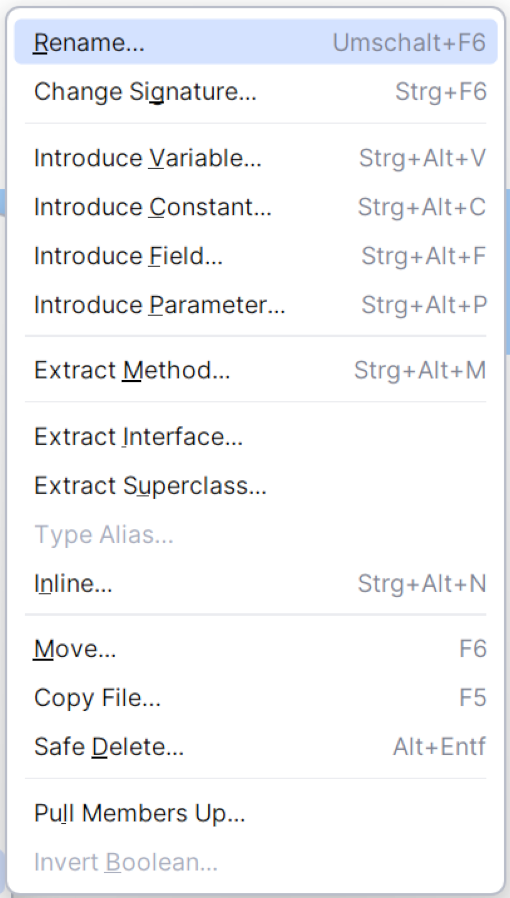
\includegraphics[width=0.35\textwidth]{Bilder/screenshotWebstorm} % Replace with your image file
  \caption{Screenshot WebStorm Refactoring-Tools \cite{webstorm.2024}}
  \label{webstormRefactor}
\end{wrapfigure}
Softwareentwicklung ist ein zeitaufwendiger Prozess, in dem es schnell zu Fehlern kommen kann. Um diese zu vermeiden, wurden verschiedenste Werkzeuge entwickelt, die die Programmierenden unterstützen sollen.
Moderne IDEs (Integrated Development Environments) haben das Ziel die Entwicklungsgeschwindigkeit zu erhöhen und Fehler zu vermeiden.
Sie kombinieren eine Vielzahl dieser hilfreichen Werkzeuge in einem einzelnen Programm. Darunter gehören unter anderem Syntax-Highlighting, Autovervollständigung, Debugging-Tools und und andere Überprüfungen, die kontinuierlich im Hintergrund laufen.
Auch Werkzeuge, die der Entwickler bewusst einsetzen kann, werden angeboten. Dazu gehören zum Beispiel Versionsverwaltung und Refactoring-Tools \citep[S. 275]{modernIDEs.2022}.\\
Die nebenstehende Abbildung \ref{webstormRefactor} zeigt das Kontextmenü für Refactoring Hilfen in der IDE WebStorm. Hier kann der Entwickler verschiedene Aktionen auswählen, die dann automatisiert durchgeführt werden.
\newpage
Ein Beispiel dafür ist die Namensänderung eines markierten Feldes. Dabei kann ein neuer Name eingegeben werden und die IDE ändert alle Stellen, an denen das Feld verwendet wird, automatisch ab.
Diese Unterstützung wird für die meisten gängigen Refactorings angeboten.\cite{webstorm.2024}
Trotzdem ist es wichtig, sich nicht vollständig auf diese Werkzeuge zu verlassen. Vorgenommene Änderungen sollten immer überprüft werden, da auch diese Tools fehlerhaft sein können \citep[S. 323 f.]{fiveLines.2023}. 

\section{Formale Verifikation der Software}
Die nächste Thematik spielt vor allem bei besonders kritischer Software eine Rolle.
Beispiele hierfür sind Systeme, von denen Menschenleben abhängen, oder bei denen erhebliche Geldsummen im Spiel sind, wie Flugzege oder der nächste Marsrover \citep[S. 324]{fiveLines.2023}.\\
Formale Verifikation beschreibt das Erheben einer Beweisführung über die Funktionstüchtigkeit von Code. Alle möglichen Ausgänge eines Programms müssen auf mathematischer Ebene bewiesen werden \cite{glinz2004formale}.
Da dieser Prozess extrem zeitaufwendig ist und Fehler in der Beweisführung unter allen Umständen vermieden werden sollten, gibt es auch hier spezielle Werkzeuge, die den Entwickler unterstützen und die Berechnungen auf Richtigkeit überprüfen.
Auch hier gilt, kommt externe Software zum Einsatz, sind Fehler dieser nicht grundsätzlich auszuschließen \citep[S. 324]{fiveLines.2023}.

\section{Eine Fehlertoleranz einbauen}
Der letzte Ansatz, der untersucht werden soll, bezieht sich auf eine gewisse Fehlertoleranz der Software.
Es gibt mehrere Möglichkeiten, diese in Code einzubauen. 
Eine davon ist das Verwenden von Feature-Schaltern. Diese können im Fehlerfall komplette Funktionaltäten deaktivieren, um die Software weiterhin lauffähig zu halten.
Alternativ kann auch ein Mechanismus eingebaut werden, der bei einem Fehler auf eine ältere stabile Version der Software zurückgreift \citep[S. 324]{fiveLines.2023}. \\
Leider gewährleistet auch dieses Vorgehen keine 100-prozentige Sicherheit, da Fehler falsch erkannt werden können.\\
\begin{singlespace}
\textit{„Ein Beispiel hierfür wäre eine Funktion, die im Fehlerfall -1 zurückgibt, anstatt einen Fehler zu werfen. Das System erwartet vielleicht eine ganze Zahl, und -1 passt zu dieser Erwartung.“} \citep[S. 324]{fiveLines.2023}.\\
\end{singlespace}
\par
Zusammenfassend lässt sich sagen, dass es viele verschiedene Möglichkeiten gibt, die Sicherheit von Software zu gewährleisten. Jedoch ist keine dieser Methoden fehlerfrei. Es ist wichtig, mehrere dieser Ansätze zu kombinieren, um die Wahrscheinlichkeit von Fehlern zu minimieren.
Diese Beobachtung speißt die Aussage, dass Software nie fertig ist, da in ihrer Lebenszeit immer wieder neue Fehler entdeckt werden, die behoben werden müssen.
    \chapter{Ungenutzte Strukturen im Code}
Im letzten Kapitel sollen einige Spezialfälle untersucht werden, bei denen oft aus verschiedenen Gründen auf ein Refactoring verzichtet wird.
Gründe dafür können unter anderem Zeitmangel, fehlende Erfahrung oder gar Faulheit der Entwickler sein.

\section{Leerzeilen nutzen}
Wenn im Code Leerzeilen verwendet werden, hat dies zumeist einen Grund. 
Programmierende grenzen dadurch Gruppierungen von Aufrufen, Variablen oder generell zusammengehörenden Codeteilen voneinander ab.
Da Leerzeilen in kürzester Zeit eingefügt werden können und einen großen Effekt zur Lesbarkeit des Codes beitragen, werden diese fast immer benutzt.
Dies ist auch ein Grund dafür, dass viele kleinere Refactorings nicht durchgeführt werden, da diese mehr Zeit in Anspruch nehmen würden. \citep[S. 325]{fiveLines.2023}
\begin{figure}[ht]
    \centering
        \begin{minted}{typescript}
function login(username: string, password: string) {
    if (username !== "admin" || password !== "123") {
        throw new Error("Invalid credentials");
    }
    const loginUser = getUser(username)

    userHistroy.push(loginUser);
    currentUser = loginUser;
}
        \end{minted}
    \caption{Loginmethode mit einer Leerzeile}
    \label{fig:LoginLeerzeile}
\end{figure}\\
Das Codebeispiel \ref{fig:LoginLeerzeile} zeigt eine stark vereinfachte Methode, um einen Login durchzuführen.
In Zeile Nr. 6 wird die Überprüfung der Anmeldedaten und die anschließende Anfrage des Nutzers, von den weiteren Bestandteilen des Logins räumlich voneinander getrennt.
Das durchzuführende Refactoring wirkt in diesem Fall fast trivial.
Die beiden Bestandteile vor und nach der Leerzeile können nach \citep[S. 325]{fiveLines.2023} in eigene Methoden gezogen werden.
Es müssen nur noch passende Funktionsnamen gewählt werden.
Das folgende Ergebnis \ref{fig:LoginErgebnis} entsteht dadurch.
\begin{figure}[ht]
    \centering
        \begin{minted}{typescript}
function updateCurrentUser(loginUser: String) {
    userHistory.push(loginUser)
    currentUser = loginUser;
}

function authenticateUser(username: String, password: string) {
    if (username !== "admin" || password !== "123") {
        throw new Error("Invalid credentials");
    }
    return getUser(username);
}

function login(username: string, password: string) {
    const loginUser = authenticateUser(username, password);
    updateCurrentUser(loginUser);
}
        \end{minted}
    \caption{Loginmethode mit extrahierten Untermethoden}
    \label{fig:LoginErgebnis}
\end{figure}
\newpage
Ein weiterer Punkt, an dem oft auf Leerzeilen zurückgegriffen wird, ist das Erstellen von Klassen.
Dort werden oft zusammengehörende Felder gruppiert.
Das folgende Codebeispiel \ref{fig:LeerzeileFelder} zeigt den Anfang einer Klasse für eine Nutzer Authentifizierung. 
\begin{figure}[ht]
    \centering
        \begin{minted}{typescript}
class Authentication{
    private username: string;
    private password: string;

    private timestamp: Date;
}
        \end{minted}
    \caption{Authentication Klasse mit einer Leerzeile}
    \label{fig:LeerzeileFelder}
\end{figure}\\
Hier kann an der 4. Zeile eine klare Einteilung zwischen den tatsächlichen Nutzerinformationen und weiteren zur Authentifizierung gehörenden Metadaten erkannt werden.
Auch in diesem Fall ist das nach \citep[S. 326]{fiveLines.2023} durchzuführende Refactoring selbsterklärend.
Der folgende Codeausschnitt \ref{fig:LeerzeileFelderErgebnis} zeigt ein mögliches Ergebnis.
\begin{figure}[ht]
    \centering
        \begin{minted}{typescript}
class UserCredentials{
    private username: string;
    private password: string;
}

class Authentication{
    private userCredentials: UserCredentials;
    private timestamp: Date;
}
        \end{minted}
    \caption{Nutzerinformationen in eigener Klasse}
    \label{fig:LeerzeileFelderErgebnis}
\end{figure}\\
\newpage
\section{Ähnlichen Code zusammenführen}
Es gibt immer wieder Situationen, in den zwei Methoden oder Klassen nahezu identisch sind, es aber trotzdem einen kleinen Unterschied gibt.
In solchen Fällen wird oft auf das Refactoring verzichtet, da der Aufwand zu groß erscheint oder die Entwickler im Programmierfluss keine einfache Lösung finden den Code zusammenzuführen.\citep[S. 326 f.]{fiveLines.2023}\\
Das folgende Beispiel zeigt zwei Klassen, die jeweils einen Formatierer umsetzen.
\begin{figure}[ht]
    \begin{subfigure}[t]{0.49\textwidth}
        \centering
        \begin{minipage}[t]{\linewidth}
            \begin{minted}[linenos=false]{typescript}
class XMLFormatter {
    format(vals: string[]) {
        let result = "";
        for (let i = 0;
              i < vals.length; i++) {
            result +=
              `<value>${vals[i]}</value>`;
        }
        return result;
    }
}
            \end{minted}
        \end{minipage}
        \caption{Klasse eines XML-Formatierers}
        \label{fig:XmlAnfang}
    \end{subfigure}
    \hfill
    \begin{subfigure}[t]{0.49\textwidth}
        \centering
        \begin{minipage}[t]{\linewidth}
            \begin{minted}[linenos=false]{typescript}
class JSONFormatter {
    format(vals: string[]) {
        let result = "";
        for (let i = 0;
              i < vals.length; i++) {
            if (i > 0) result += ",";
            result +=
                `{ value: "${vals[i]}" }`;
        }
        return result;
    }
}
            \end{minted}
        \end{minipage}
        \caption{Klasse eines JSON-Formatierers}
        \label{fig:JsonAnfang}
    \end{subfigure}
    \caption{Ähnliche Formatierer Klassen \citep[S. 327]{fiveLines.2023}}
    \label{fig:FormatterAnfang}
\end{figure}\\
Vergleicht man die beiden Klassen \ref{fig:XmlAnfang} und \ref{fig:JsonAnfang}, fällt auf, dass diese nahezu identisch sind.
Ein Unterschied ist zum Einen die abweichende Formatierung jedes einzelnen Wertes.
Bei XML wird der Wert in ein Tag eingebettet, bei JSON wird ein Objekt mit einem Schlüssel-Wert-Paar in geschweiften Klammern erstellt.
Dieser Unterschied liese sich einfach vereinen, da dort nur unterschiedliche Zeichenketten eingefügt werden müssen.
Die ausschlaggebende Problematik stellt das trennende Komma zwischen einzelnen Werten, im JSON Format, dar.
Dies verhindert eine einfache Zusammenführung der beiden Klassen.
Da das Refactoring aus mehreren kleinen, aber einfachen Schritten besteht, betrachten wir das in der nachfolgenden Abbildung \ref{fig:FormatterEnde} gezeigte Ergebnis.

\begin{figure}[ht]
    \begin{subfigure}[t]{0.49\textwidth}
        \centering
        \begin{minipage}[t]{\linewidth}
            \begin{minted}[linenos=false]{typescript}
class XMLFormatter {
    format(vals:string[]) {
        return new Formatter(
            new FormatSingle
                ("<value>", "</value>"),
            new None()).format(vals);
    }
}
class JSONFormatter {
    format(vals:string[]) {
        return new Formatter(
            new FormatSingle
                ("{ value: '", "' }"),
            new Comma()).format(vals);
    }
}
class Formatter {
    constructor(
        private single: FormatSingle,
        private sep: Seperator) { }
    format(vals: string[]) {
        let result = "";
        for (let i=0; i < vals.length; i++) 
        {
            reuslt = 
              this.sep.put(i,result);
            result += 
              this.single.format(vals[i]);
        }
        return result;
    }
}
            \end{minted}
        \end{minipage}
        \caption{Formattierer Klassen}
        \label{fig:gleichGut1}
    \end{subfigure}
    \hfill
    \begin{subfigure}[t]{0.49\textwidth}
        \centering
        \begin{minipage}[t]{\linewidth}
            \begin{minted}[linenos=false]{typescript}
class FormatSingle {
    constructor(
        private before: string,
        private after: string) { }
    format(val: string) {
        return `${prefix}${val}${after}`
    }
}

class Seperator {
    put(i: number, result: string): string;
}
class Comma implements Seperator {
    put(i: number, result: string) {
        if (i > 0) result += ",";
        return result;
    }
}
class None implements Seperator {
    put(i: number, result: string) {
        return result;
    }
}
            \end{minted}
        \end{minipage}
        \caption{Seperator Klassen}
        \label{fig:gleichGut2}
    \end{subfigure}
    \caption{Ergebnis der Formatierer nach Refactoring \citep[S. 329 f.]{fiveLines.2023}}
    \label{fig:FormatterEnde}
\end{figure}
\newpage
Bei der Betrachtung der Klasse \textit{Formatter} fällt auf, dass diese eine große Ähnlichkeit zu den beiden ursprünglichen Klassen aufweist.
Der Unterschied besteht darin, dass im Konstruktor zwei weitere Klassen übergeben werden, die das Formatieren der einzelnen Werte und das Einfügen des trennenden Kommas übernehmen.\\
Die erste Klasse \textit{FormatSingle} übernimmt die genereller Formatierung einer Eingabe. Sie kann mit zwei beliebigen Zeichenketten instanziiert werden, die jeweils vor und nach dem eigentlichen Wert eingefügt werden.\\
Die Zweite, \textit{Seperator}, übernimmt das Einfügen eines trennenden Zeichens zwischen den einzelnen Werten. Bei der Klasse \textit{Comma} wird ein Komma eingefügt, wenn der Index größer als 0 ist. Die Klasse \textit{None} fügt kein Zeichen ein.\\
Abschließend müssen noch die jeweiligen Klassen, \textit{XMLFormatter} und \textit{JSONFormatter}, mit den jeweils richtigen Werten instanziiert werden.\\

Das Ergebnis dieses Refactorings ist eine deutlich verbesserte Struktur, die die Wartbarkeit und Erweiterbarkeit des Codes deutlich erhöht. Es können ohne Probleme weitere Implementierungen von Formatierern erstellt werden, die nach ähnlichen Mustern arbeiten. 
\section{Gemeinsame Affixe nutzen}
Ein weiteres eindeutiges Merkmal, für ein klares Refactoring, ist die Verwendung von gemeinsamen Affixen in Methoden- oder Klassennamen.
Dies deutet darauf hin, dass diese Codeteile eine klare Zusammengehörigkeit haben und in eine gemeinsame Struktur gekapselt werden können.
Laut der Regel \textbf{\textit{„Vermeide gemeinsame Affixe“}}, können alle Felder und Methoden mit gleichem Präfix oder Suffix in eine eigene Klasse oder ein eigenes Interface extrahiert werden.
Das Affix wird dabei zum Namen der neu erstellten Struktur \citep[S. 201 ff.]{fiveLines.2023}.\\
Das folgende Beispiel zeigt Code, bei dem sofort auffällt, dass diese Regel verletzt wird. 
\begin{figure}[ht]
    \centering
        \begin{minted}{typescript}
interface Protocol {...}
class StringProtocol implements Protocol {...}
class JSONProtocol implements Protocol {...}
class ProtobufProtocol implements Protocol {...}
/// ...
    let p = new StringProtocol();
/// ...
        \end{minted}
    \caption{Codeausschnitt mit gemeinsamen Suffix \citep[S. 331]{fiveLines.2023}}
    \label{fig:AffixeSchlecht}
\end{figure}\\
Wird der Code betrachtet, fällt auf, dass \textit{„Protocol“} in allen Klassennamen vorkommt.
Der Grund warum Programmierende dieses Refactoring in diesem Fall nicht durchführen, wird klar, wenn das Ergebnis betrachtet wird.
Entfernt man bei der Klasse \textit{StringProtocol} das Suffix, bleibt nur noch \textit{„String“} übrig.
Dies steht in Konflikt mit einer Basisklasse der Programmiersprache \citep[S. 330 f.]{fiveLines.2023}.
Um diese Codestelle trotzdem zu verbessern, kann das Refactoring in leicht abgeänderter Form durchgeführt werden.
Wie im folgenden Codebeispiel \ref{fig:AffixeGut} gezeigt, kann das Problem mithilfe eines \textit{„Namespace“} gelöst werden.
\begin{figure}[ht]
    \centering
        \begin{minted}{typescript}
namespace ptotocol {
    export interface Protocol {...}
    export class String implements Protocol {...}
    export class JSON implements Protocol {...}
    export class Protobuf implements Protocol {...}
}

/// ...
    let p = new protocol.String();
/// ...
        \end{minted}
    \caption{Codeausschnitt mit Namespace \citep[S. 331]{fiveLines.2023}}
    \label{fig:AffixeGut}
\end{figure}\\
Dieser Ansatz ist zwar zielführend, trotzdem sollte hier von Fall zu Fall entschieden werden, ob es eine bessere Lösung gibt, dies zu lösen.
Da \textit{„String“} eine häufig verwendete Klasse ist, erschwert das gezeigte Beispiel die Nutzbarkeit des Codes weiter und ist nicht sinnvoll.
\section{Den Laufzeittyp bearbeiten}
Das letzte Beispiel, das betrachtet werden soll, zeigt eine Situation bei der auf den Operator \textit{\textbf{„instanceof“}} zurückgegriffen wird, um abhängig davon verschiedene Aufrufe ausgeführt werden sollen.
Die Unterscheidung wird mithilfe von \textit{\textbf{„if“}}-Abfragen durchgeführt. Laut Clausen sollten \textit{\textbf{„if“}}-Anweisungen in Kombination mit \textit{\textbf{„else“}} vermieden werden.
Nur Fälle mit \textit{\textbf{„instanceof“}}, \textit{\textbf{„typeof“}} oder Casts werden als Ausnahme genannt. \citep[S. 332]{fiveLines.2023}\\
Das folgende Beispiel \ref{fig:LaufzeitSchlecht} zeigt solch eine Situation.

\begin{figure}[ht]
    \centering
        \begin{minted}{typescript}
function foo(obj: any) {
    if (obj instanceof A) {
        obj.methodA();
    } else if (obj instanceof B) {
        obj.methodB();
    }
}
class A {
    methodA() { ... }
}
class B {
    methodB() { ... }
}
        \end{minted}
    \caption{\textit{if}-Anweisung mit \textit{instanceof} \citep[S. 331]{fiveLines.2023}}
    \label{fig:LaufzeitSchlecht}
\end{figure}
In der Funktion \textit{foo} wird überprüft, ob das übergebene Objekt eine Instanz der Klasse \textit{A} oder \textit{B} ist.
Abhängig vom Ergebnis werden dann ihre jeweiligen Methoden aufgerufen.
Dieses Verhalten ist ein Paradebeispiel für die Nutzung eines Interfaces.\\
\begin{singlespace}
\textit{„Interfaces erlauben es uns, einer Variablen Objekte verschiedener Klassen zuzuweisen. Wenn wir dann eine Methode daran aufrufen, wird der Aufruf zur richtigen Klasse geleitet. Gleichzeitig ist das auch der Weg, wie wir Typenuntersuchungen zur Laufzeit vermeiden können.“} \citep[S. 332]{fiveLines.2023}\\
\end{singlespace}
\newpage
Das folgende Beispiel \ref{fig:LaufzeitGut} zeigt, wie das Problem mit dem erklärten Ansatz gelöst werden kann.
\begin{figure}[ht]
    \centering
        \begin{minted}{typescript}
function foo(obj: Foo) {
    obj.foo();
}
class A implements Foo {
    foo() {
        this.methodA();
    }
    methodA() { ... }
}
class B implements Foo {
    foo() {
        this.methodB();
    }
    methodB() { ... }
}
interface Foo {
    foo(): void;
}
        \end{minted}
    \caption{Refactoring mit Interface \citep[S. 332 f.]{fiveLines.2023}}
    \label{fig:LaufzeitGut}
\end{figure}\\
Abschließend lässt sich sagen, dass Refactoring in den gezeigten Situationen oft zu einer besseren Codebasis führt. Auch wenn es im Moment des Programmierens nicht sinnvoll wirkt, sollte der kleine Mehraufwand in Kauf genommen werden.
Es ist wichtig, dass Entwickler sich immer wieder bewusst machen, dass Code nicht nur für den Moment geschrieben wird, sondern auch in Zukunft noch wartbar und erweiterbar sein sollte.
Müssen andere Entwickler im Nachgang den Code anpassen, nimmt dies mehr Zeit in Anspruch, als wenn der Code von Anfang an sauber strukturiert ist.
    \chapter{Fazit}
Abschließend lässt sich sagen, dass Refactoring ein wichtiger Bestandteil der Softwareentwicklung ist.
Es hilft dabei, die Qualität und Wartbarkeit von Code zu verbessern und somit die Lebensdauer von Software zu verlängern.\\
Das Seminar hat gezeigt, dass Strukturen im Code eine wichtige Rolle spielen und Verhalten in verschiedenen Formen abgebildet werden kann.
Auch das Vezichten auf Refactoring kann in manchen Fällen sinnvoll sein, um die Entwicklung nicht zu verlangsamen, auch wenn es auf den ersten Blick nicht so wirkt.
Ein weiterer wichtiger Punkt ist die Sicherheit von Software. Diese kann durch Tests, Werkzeuge, formale Verifikation und Fehlertoleranz gewährleistet werden.\\


% ----------------------------------------------
\backmatter 

\printbibliography[heading=bibintoc]

\newpage
\thispagestyle{empty}

% Bitte hier keine Änderungen vornehmen, sondern vollständig handschriftlich ausfüllen

\noindent  {\Large \textbf{Erklärung}}\\ 

\vspace*{2cm}

\noindent
Hiermit versichere ich, dass ich die vorliegende Arbeit selbstständig angefertigt, 
nicht anderweitig für Prüfungszwecke vorgelegt, alle benutzten
Quellen und Hilfsmittel angegeben, sowie wörtliche und sinngemäße Zitate gekennzeichnet habe.
\vspace{2cm}

\noindent
Füssen, den 27. Juni 2023
\hspace*{2cm}%
\dotfill\\
\hspace*{8.5cm}%
\textit{Unterschrift des Verfassers}

% \vspace*{5cm}

% \noindent  {\Large \textbf{Ermächtigung}}\\ 

% \vspace*{2cm}

% \noindent
% Hiermit ermächtige ich die Hochschule Kempten zur Veröffentlichung der Kurzzusammen-
% fassung (Abstract) meiner Arbeit, z. Bsp. auf gedruckten Medien oder auf einer Internet-
% seite.
% \vspace{2cm}

% \noindent
% Ort, den 01. Januar 2100
% \hspace*{2cm}%
% \dotfill\\
% \hspace*{8.5cm}%
% \textit{Unterschrift des Verfassers}
 	% Erklärungen - Unterschreiben nicht vergessen!

\end{document}

% Vorlage erstellt von Alexander Bartel (alexander.bartel@hs-kempten.de), Fakultät Informatik, Hochschule Kempten (c) CC BY 4.0
% ergänzt durch: Prof. Dr. Rieck (stefan.rieck@hs-kempten.de)
% 20230329 SR umgestellt auf biblatex und biber
